\section{Method of characteristics}
\label{sec:moc}

Path~B develops the analytical ladder for probability generating functions of continuous-time absorption models. Section~\ref{sec:pgf-bridge} already recorded the univariate linear birth--death case: the master equation compresses to a first-order PDE, solved along characteristics. Here the state is bivariate---intracellular and extracellular counts---and the transitions are absorption, death, and birth. The same idea applies: write the forward equations, pass to a generating function $G(x,y,t)$, obtain a first-order PDE, and integrate along characteristics.

The original motivation is multi-host pathogenesis: once a cell ruptures, a large extracellular cohort becomes available for absorption by the remaining hosts. As a step towards that picture one studies single-host ``absorption models'', in which a pathogenic cohort moves from the medium into one cell, with or without intracellular birth and death. Immediate whole-cohort transfer between cells is a harder assumption to defend; absorption over an intermediate period is more realistic. The calculations below supply the generating-function technology for those building blocks.

\subsection{Only absorption}
The simplest absorption process is a single host cell that takes up pathogenic particles but in which no subsequent dynamics occur --- neither birth nor death of pathogen within the host.

Let $\xt$ and $\yt$ denote the number of pathogenic particles within and outside the host cell respectively; the same labelling is used in the later versions of the single-host model. Events are assumed throughout to be stochastic, separated by exponentially distributed inter-event times, a property that follows from taking event rates to be time-independent. Our continuous-time stochastic process $\{(\xt, \yt) : t\in[0,\infty)\}$ therefore conforms to the memoryless Markov property.

With only absorption to consider, the model is specified by the following probabilities --- outcome-likelihoods over an infinitesimal duration, $\Delta t$ (taken in the limit to 0).
%\begin{equation}
  % \begin{split}
  %   \pr{\Delta\xx= 1,\;\Delta\yy = -1 \;|\; \yt = j} = j \alpha \Delta t\\
 %    \pr{\Delta\xx= 0,\;\Delta\yy = 0 \;|\; \yt = j} = 1 -  j \alpha \Delta t
 %  \end{split}
%\label{probSpec1}
%\end{equation}
\begin{align*}
     \pr{\Delta\xx= 1,\;\Delta\yy = -1 \;|\; \yt = j} &= j \alpha \Delta t,  &&\text{(absorption)}\\
     \pr{\Delta\xx= 0,\;\Delta\yy = 0 \;|\; \yt = j} &= 1 -  j \alpha \Delta t,  &&\text{(no event)}
\end{align*}


\noindent
Here $\Delta \xx = \xx_{t+\Delta t} - \xt$ (and likewise for $\yy$). Notice the multiplication by $j$, the number of extracellular particles: each unit is subject to the same probability, $\alpha \Delta t$, of being taken up.

The initial condition is fixed as $\xx_0 = 0$, $\yy_0 = N$ --- a starter population of census $N$ occupying the extracellular medium.

Defining state probabilities, $p_{i,j}(t) = \pr{\xt = i,\; \yt = j}$, we can write down the forward Kolmogorov equations:
\begin{equation}
\label{F1}
\ddt{\p} = \alpha(j + 1) p_{i-1,j+1} - \alpha j \p.
\end{equation}

\noindent
Then, with the probability generating function defined,
\begin{equation}
\label{pgfDef}
G(x,y,t) = \sum_i\sum_j \pt x^iy^j
\end{equation}

\noindent
$\left(=\mathbb{E}\left[x^{\xt}y^{\yt}\right]\right)$, we can derive a PDE for $G(x,y,t)$ in the following way.

First, multiply each equation in (\ref{F1}) by $x^iy^j $,
\begin{equation*}
%\label{pdeDerev1}
\pddt{\p x^iy^j} = \alpha(j + 1) p_{i-1,j+1}x^iy^j - \alpha j \p x^iy^j.
\end{equation*}

\noindent
Then sum over $i$ and $j$ for non-zero $\pt$,
\begin{equation}
\label{pdeDere2}
\sum_{i = 0}^N\sum_{j=0}^N\pddt{\p x^iy^j} = \alpha\sum_{i = 1}^{N+1}\sum_{j=-1}^{N-1}(j + 1) p_{i-1,j+1}x^iy^j - \alpha \sum_{i = 0}^N\sum_{j=0}^Nj \p x^iy^j.
\end{equation}

\noindent
(Note, for any $i, j > N$, and when $i+j \neq N$, $\pt = 0$ $\forall t$. This is because pathogenic particles in this model are neither created nor destroyed.)

Rearranging (\ref{pdeDere2}), we find
\begin{equation*}
\label{pdeDerev2}
\sum_{i = 0}^N\sum_{j=0}^N\pddt{\p x^iy^j} = \alpha\left(x\sum_{i = 0}^N\sum_{j=0}^N j p_{i,j}x^{i}y^{j-1} -  y\sum_{i = 0}^N\sum_{j=0}^Nj \p x^iy^{j-1} \right),
\end{equation*}

\noindent
which can be written in terms of the following partial derivatives,
\begin{equation*}
\label{pdeDerev2b}
\sum_{i = 0}^N\sum_{j=0}^N\pddt{\p x^iy^j} = \alpha\left(x - y\right)\sum_{i = 0}^N\sum_{j=0}^N \pdd{\p x^iy^j}{y}.
\end{equation*}

\noindent
Notice, with (\ref{pgfDef}),
\begin{equation}
\label{PDE1}
\pddt{G(x,y,t)} = \alpha\left(x - y\right) \pdd{G(x,y,t)}{y};
\end{equation}

\noindent
the chosen initial condition corresponding to $G(x,y,0) = y^N$.

This first-order linear initial value problem, it turns out, proves quite difficult to solve. The method of characteristics, though practicable by definition on equations of three variables, is not elementary by inspection here. As it happens, though, we can obtain the solution by other means.

\subsubsection*{Benefits of the independence property}
The function $G(x,y,t)$ referred to above was specific to the initial condition $\xx_0 = 0$, $\yy_0 = N$. It helps to carry that starting state explicitly in the notation,
\begin{equation*}
G_n(x,y,t) = \sum_i\sum_j \pr{\xt = i,\;\yt=j \;|\;\xx_0 = 0,\;\yy_0=n } x^i y^j.
\end{equation*}
In a process of absorption alone, each of the $N$ pathogenic particles gets taken up by the host cell one by one, and a single particle of the cohort behaves without reference to the movements of its neighbours. Because of this independence, our variables $\xt$ \& $\yt$ can be thought of as the sum of $N$ sub-variables, $\xt^{(k)}$ \& $\yt^{(k)}$, each pertaining only to the movements of a single pathogenic unit:
\begin{align*}
\xt = \xt^{(1)} + \xt^{(2)} + \dots + \xt^{(n)}\\
\yt = \yt^{(1)} + \yt^{(2)} + \dots + \yt^{(n)}
\end{align*}
This observation allows us to prove that
\begin{equation}
\label{indRelPGF}
G_n(x,y,t) = \lrb{G_1(x,y,t)}^n:
\end{equation}
\begin{align*}
G_n(x,y,t) &= \ex{x^{\sum_{k=1}^n \xt^{(k)}} y^{\sum_{k=1}^n \yt^{(k)}}}\\
&=  \ex{\prod_{k=1}^n x^{\xt^{(k)}} \prod_{k=1}^n y^{\yt^{(k)}} }\\
&=  \prod_{k=1}^n\ex{ x^{\xt^{(k)}} y^{\yt^{(k)}} }\\
&=  \prod_{k=1}^n G_1(x,y,t)\\
&= \left(G_1(x,y,t)\right)^n
\end{align*}

\noindent
Now consider a system with only one pathogenic particle to begin with; $\xx_0 = 0$, $\yy_0 = 1$. It would after some time be absorbed, and this would be the final state of the system. No other states could be reached --- quite simply: $\pt = 0$ $\forall t$ for $i+j \neq1$.\par
The state probabilities of this simple case can hence be fully determined from the forward Kolmogorov equations.
\begin{align*}
\ddt{p_{0,1}(t)} = -\alpha p_{0,1}(t) && \ddt{p_{1,0}(t)} = \alpha p_{0,1}(t)
\end{align*}
$\implies$
\begin{align*}
p_{0,1}(t) = \ee^{-\alpha t} && p_{1,0}(t) = 1 - \ee^{-\alpha t}
\end{align*}



\begin{figure}[H]
\begin{center}
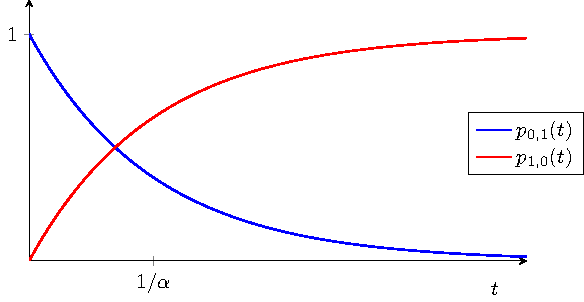
\includegraphics[width = 0.65\textwidth]{figures/IMG_ch3/abs1.pdf}
\end{center}
\end{figure}



\noindent
Given that these are the only two non-zero state probabilities of the single-particle system, we can write out the associated probability generating function as
\begin{align*}
G_1(x,y,t) &= p_{1,0}(t)x + p_{0,1}(t)y\\
    &=   \lrb{1-\ee^{-\alpha t} }x + \ee^{-\alpha t}y.
\end{align*}
Applying relation (\ref{indRelPGF}) then defines the probability generating function for this absorption-only system generally, for any initial state,
\begin{equation*}
G_n(x,y,t) = \lrb{ \lrb{1-\ee^{-\alpha t} }x + \ee^{-\alpha t}y}^n;
\end{equation*}

\noindent
which does satisfy equation (\ref{PDE1}) along with its initial condition,
$$G_n(x,y,0) = y^n.$$


%- forward kolmogorov equations

%- PDE for probability generating function

%- note on difficulty in solving it

%- Solution allowed by independence assumption.


\subsection{Absorption-death}

In reality, pathogenic particles resident in a host cell may be subject to death. \par
Setting up a model as above, with $\xt$ \& $\yt$ representing the count of intracellular and extracellular pathogen, we can incorporate particle death with the following addition.
\begin{align*}
     \pr{\Delta\xx= 1,\;\Delta\yy = -1 \;|\; \yt = j} &= j \alpha \Delta t,  &&\text{(absorption)}\\
      \pr{\Delta\xx= -1,\;\Delta\yy = 0 \;|\; \xt = i} &= i \mu \Delta t,  &&\text{(death)}\\
     \pr{\Delta\xx= 0,\;\Delta\yy = 0 \;|\; \yt = j, \xt=i} &= 1 -  \lrb{ j\alpha + i\mu}\Delta t,  &&\text{(no event)}
\label{probSpec1}
\end{align*}

From here an analogous line of reasoning can be followed, and a familiar difficulty is met on arrival at the first order linear PDE,
\begin{equation*}
\label{PDE2}
\pddt{G(x,y,t)} = \mu(1-x) \pdd{G(x,y,t)}{x}+\alpha\left(x - y\right) \pdd{G(x,y,t)}{y}.
\end{equation*}

\noindent
This point being reached from a similar derivation using the forward Kolmogorov equations:
\begin{equation*}
\label{FK1}
\ddt{\p} = \alpha(j + 1) p_{i-1,j+1} + \mu(i+1)p_{i+1,j} - (\alpha j + \mu i) \p.
\end{equation*}

\noindent
But as above, the solution can be constructed with a work-around employing the relation
\begin{equation*}
G_n(x,y,t) = \lrb{G_1(x,y,t)}^n.
\end{equation*}

\noindent
As before, individual particles are independent from one another in their movements.\par
Without birth events, the maximum number of particles in the system is restricted to its initial value. So, when considering the case of an isolated pathogenic unit, the probability generating function takes its form,
\begin{equation*}
G_1(x,y,t) = p_{0,0} + p_{1,0}x + p_{0,1}y.
\end{equation*}

\noindent
These state-probabilities can be determined as follows using the forward Kolmogorov equations.
\begin{align*}
\ddt{p_{0,1}(t)} = -\alpha p_{0,1}(t) && \ddt{p_{1,0}(t)} = \alpha p_{0,1}(t) - \mu p_{1,0}(t)
\end{align*}
$\implies$
\begin{align*}
p_{0,1}(t) = \ee^{-\alpha t} && p_{1,0}(t) = \frac{\alpha}{\mu - \alpha} \Big(   \ee^{-\alpha t} - \ee^{-\mu t} \Big) && p_{0,0}(t) = 1 -p_{0,1}(t)  -p_{1,0}(t)
\end{align*}



\begin{figure}[H]
\begin{center}
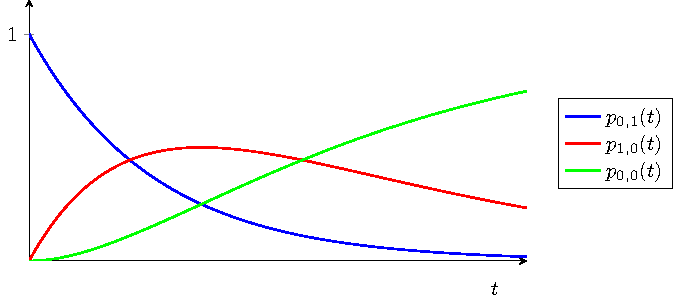
\includegraphics[width = 0.65\textwidth]{figures/IMG_ch3/abs2.pdf}
\end{center}
\caption{Characteristic geometry for the absorption--death model.}
\end{figure}





\noindent
Relation (\ref{indRelPGF}) then leads, as above, to the general probability generating function, $G_n(x,y,t)$:
\begin{equation*}
G_n(x,y,t) = \lrb{1-\frac{\mu}{\mu - \alpha}  \ee^{-\alpha t}  + \frac{\alpha}{\mu - \alpha} \ee^{-\mu t}  + \frac{\alpha}{\mu - \alpha} \Big(   \ee^{-\alpha t} - \ee^{-\mu t} \Big)x +  \ee^{-\alpha t} y}^n
\end{equation*}



%\begin{equation}
%G_1(x,y,t) = 1-\frac{\mu}{\mu - \alpha}  \ee^{-\alpha t}  + \frac{\alpha}{\mu - \alpha} \ee^{-\mu t}  + \frac{\alpha}{\mu - \alpha} \Big(   \ee^{-\alpha t} - \ee^{-\mu t} \Big)x +  \ee^{-\alpha t} y
%\end{equation}

\subsection{Method of characteristics (absorption-death)}

Before continuing to the case of absorption-birth-death, where replication may occur within the host cell, let us revisit absorption-death from the point of its PDE for $G(x,y,t)$.

\begin{equation}
\label{PDE2b}
\pddt{G(x,y,t)} = \mu(1-x) \pdd{G(x,y,t)}{x}+\alpha\left(x - y\right) \pdd{G(x,y,t)}{y},
\end{equation}
with initial condition $G(x,y,0) = y^N$.

The method of characteristics is the standard tool for first-order linear PDEs of this type for 3 variate problems.\par
We begin by introducing a change of variables $(x,y,t) \to (s,r,\tau)$:
$$G(x,y,t) = G\big(x(s,r,\tau), y(s,r,\tau), t(s,r,\tau) \big) \equiv G(s,r,\tau)$$
The method works by seeking solutions on the characteristic surfaces of constant $s$ and $r$; $G(\tau)$. To do so, we must introduce an initial surface in the $s$, $r$, $\tau$ space:
\begin{align}
\label{ICpar}
x(s,r,0) = s && y(s,r,0) = r && t(s,r,0) = 0
\end{align}

With the probability generating function now a function of only one variable, $\tau$, we can write down the characteristic equations as ODEs. First, consider,
\begin{equation*}
\dda{G}{\tau} = \pddt{G} \dda{t}{\tau}  +  \pdd{G}{x}\dda{x}{\tau} + \pdd{G}{y}\dda{y}{\tau} .
\end{equation*}
Notice similarity with (\ref{PDE2}),
$$0  = -\pddt{G} + \mu(1-x)\pdd{G}{x} + \alpha (x-y)\pdd{G}{y}.$$
Comparing coefficients, we can write down the characteristic ODEs:
\begin{align}
\dda{G}{\tau} &= 0\label{ch11}\\
\dda{t}{\tau} &= -1\label{ch12}\\
\dda{x}{\tau} &= \mu(1-x)\label{ch13}\\
\dda{y}{\tau} &= \alpha(x-y)\label{ch14}
\end{align}


\subsubsection*{(\ref{ch11})}
Solving the first characteristic equation,
$$\dda{G}{\tau} = 0$$
$$G = \phi(s,r)$$
$\phi$ constant on surfaces of constant $s$, and $r$.\par
With  (\ref{ICpar}), the initial condition on $G$ translates to $G(s,r,\tau=0) = r^N$, which informs us that $\phi(s,r) = r^N$. Hence,
\begin{equation}
\label{GrN}
G(s,r,\tau) = r^N.
\end{equation}



\subsubsection*{(\ref{ch12})}
$$\dda{t}{\tau} = -1$$
$$t = -\tau + c(s,r)$$
Using (\ref{ICpar}), we can fix the constant, $c(s,r) = 0$.
\begin{equation}
\label{minustau}
t = -\tau
\end{equation}


\subsubsection*{(\ref{ch13})}
$$\dda{x}{\tau} = \mu(1-x)$$
$$\vdots$$
$$1-x = c(s,r) \ee^{-\mu \tau}.$$
With initial condition, (\ref{ICpar}), $c(s,r) = 1-s$;
\begin{equation}
\label{sandxwithtau}
1-x = (1-s) \ee^{-\mu \tau}.
\end{equation}


\subsubsection*{(\ref{ch14})}

\begin{align*}
\dda{y}{\tau} &= \alpha(x-y)\\
\dda{y}{\tau} &= \alpha\left(1-(1-s) \ee^{-\mu \tau} -y\right)
\end{align*}
$$\vdots$$
$$y = 1 - \frac{\alpha}{\alpha-\mu}(1-s)\ee^{-\mu\tau} + c(s,r)\ee^{-\alpha\tau}.$$
Applying (\ref{ICpar}), $c(s,r) = r + \frac{\alpha}{\alpha-\mu}(1-s) -1$;
\begin{equation}
\label{ywithr1}
y = 1 - \frac{\alpha}{\alpha-\mu}(1-s)\ee^{-\mu\tau} + \lrb{r + \frac{\alpha}{\alpha-\mu}(1-s) -1}\ee^{-\alpha\tau}.
\end{equation}

\vspace{15pt}
\noindent
Finally, if we rearrange (\ref{ywithr1}) for $r$, also substituting $s(x,y,t)$ from (\ref{sandxwithtau}), and $\tau = -t$ from (\ref{minustau}), we find:
\begin{equation*}
r = 1-\frac{\mu}{\mu - \alpha}  \ee^{-\alpha t}  + \frac{\alpha}{\mu - \alpha} \ee^{-\mu t}  + \frac{\alpha}{\mu - \alpha} \Big(   \ee^{-\alpha t} - \ee^{-\mu t} \Big)x +  \ee^{-\alpha t} y
\end{equation*}
Then, with $G = r^N$ ((\ref{GrN})), this matches the solution obtained in the previous section,
\begin{equation*}
G(x,y,t) = \lrb{1-\frac{\mu}{\mu - \alpha}  \ee^{-\alpha t}  + \frac{\alpha}{\mu - \alpha} \ee^{-\mu t}  + \frac{\alpha}{\mu - \alpha} \Big(   \ee^{-\alpha t} - \ee^{-\mu t} \Big)x +  \ee^{-\alpha t} y}^N.
\end{equation*}



\subsection{Absorption-birth-death}

Introducing replication for particles inside the host cell, we will see that though the independence property is still present, it no longer serves as a work-around in finding the probability generating function $G(x,y,t)$. This is because, given a single initial infectious particle, with birth events an infinite number of states can be reached; hence $G_1(x,y,t)$ will be constituted by an infinite number of terms.\par

We are now equipped, however, to solve the PDE for $G(x,y,t)$ directly, and this is the approach we will take.\par

Setting up the model like in previous cases, $\xt$ \& $\yt$ represent the counts of intracellular and extracellular pathogenic particles. Birth events are added to the transition rates as follows.

\begin{align*}
     \pr{\Delta\xx= 1,\;\Delta\yy = -1 \;|\; \yt = j} &= j \alpha \Delta t,  &&\text{(absorption)}\\
     \pr{\Delta\xx= 1,\;\Delta\yy = 0 \;|\; \xt = i} &= i \beta \Delta t,  &&\text{(birth)}\\
      \pr{\Delta\xx= -1,\;\Delta\yy = 0 \;|\; \xt = i} &= i \mu \Delta t,  &&\text{(death)}\\
     \pr{\Delta\xx= 0,\;\Delta\yy = 0 \;|\; \yt = j, \xt=i} &= 1 -  \lrb{ j\alpha + i\mu + i\beta}\Delta t,  &&\text{(no event)}
\label{probSpec1}
\end{align*}

The forward Kolmogorov equation is written as such.
\begin{equation*}
\label{FK3}
\pddt{\p } = \alpha(j + 1) p_{i-1,j+1} + \mu(i+1)p_{i+1,j}  +  \beta(i-1)p_{i-1,j}    -  (\alpha j + \mu i+\beta i) \p
\end{equation*}

From here, again with the reasoning seen above, we can derive the associated PDE for $G(x,y,t)$.

\begin{equation}
\pddt{G} = \lrb{\mu - (\mu+ \beta)x + \beta x^2}\pdd{G}{x} + \alpha(x-y)\pdd{G}{y}
\end{equation}

To solve this by the method of characteristics we again re-parametrise $(x,y,t)$ as $(s,r,\tau)$, then seek solutions on characteristic surfaces of constant $s$ and $r$. Doing so brings us to the characteristic ODEs:
\begin{align}
\dda{G}{\tau} &= 0\label{ch21}\\
\dda{t}{\tau} &= -1\label{ch22}\\
\dda{x}{\tau} &= \mu-(\mu+\beta)x + \beta x^2\label{ch23}\\
\dda{y}{\tau} &= \alpha(x-y)\label{ch24}
\end{align}
Applying the same initial conditions on $(s,r,\tau)$ as above in (\ref{ICpar}), we can solve these equations as follows.

\subsubsection*{(\ref{ch21}) \& (\ref{ch22})}
Like in the previous section the first two characteristic equations yield:
$$G(s,r,\tau) = \phi(s,r),$$
and ultimately,
\begin{equation}
\label{gngngn}
G(s,r,\tau) = r^N.
\end{equation}
Then,
$$t = -\tau.$$


\subsubsection*{(\ref{ch23})}
This equation has the same structural shape as the survival recurrence for $S_n$ in the discrete branching section, the survival probability.
$$\dda{x}{\tau} = \beta\lrb{x-x_+}\lrb{x-x_-}$$
with,
$$x_{\pm} = \frac{\mu + \beta}{2\beta} \pm \sqrt{\lrb{\frac{\mu + \beta}{2\beta}}^2 - \frac{\mu}{\beta}}.$$
The main difference in its solution with the discrete survival recurrence comes with an $s$ when fixing the constant of integration:
\begin{equation}
x(\tau) = \frac{x_+(s-x_-) - x_-(s-x_+)\ee^{\beta(x_+-x_-)\tau}}{(s-x_-) - (s-x_+)\ee^{\beta(x_+-x_-) \tau}}
\label{xabd}
\end{equation}


\subsubsection*{(\ref{ch24})}
The last characteristic equation is
$$\dda{y}{\tau} = \alpha(x-y).$$
To solve this we will need to substitute $x$ as found above, (\ref{xabd}). With an integrating factor, the equation becomes,
$$\dda{}{\tau}\lrb{\ee^{\alpha\tau} y} = \alpha \ee^{\alpha\tau} x(\tau).$$
Integrating with respect to $\tau$,
$$\ee^{\alpha\tau }y = \alpha\int \ee^{\alpha\tau} \frac{x_+(s-x_-) - x_-(s-x_+)\ee^{\beta(x_+-x_-)\tau}}{(s-x_-) - (s-x_+)\ee^{\beta(x_+-x_-) \tau}} \dd\tau.$$
Then splitting the numerator,
\begin{align}
\label{bigdoubleints}
\ee^{\alpha\tau }y &=  \alpha x_+(s-x_-) \int \frac{ \ee^{\alpha \tau} } {(s-x_-) - (s-x_+)\ee^{\beta(x_+-x_-) \tau}}\dd\tau \notag \\
&-\alpha x_-(s-x_+)\int\frac{\ee^{\left[ \alpha + \beta(x_+-x_-) \right]\tau}}{(s-x_-) - (s-x_+)\ee^{\beta(x_+-x_-) \tau}}\dd\tau.
\end{align}

\noindent
Each of these integrals can be written in the form,
\begin{equation*}
I(\tau) = \int\frac{\ee^{h\tau}}{p+q\ee^{k\tau}}\dd\tau.
\end{equation*}
where $h$, $k$, $p$, $q$ are all constants. For example, in the first integral, $h = \alpha$, $k = \beta(x_+ - x_-)$, $p = (s-x_-)$, and $q = -(s-x_+)$. As it happens, we can solve this integral with:
\begin{equation}
\label{hypIden}
I(\tau) = \frac{\ee^{h\tau}}{ph} {}_2F_1\lrb{1,\frac{h}{k};\frac{h}{k}+1; -\frac{q}{p}\ee^{k\tau}} + \text{const}.
\end{equation}
${}_2F_1(a,b;c;z)$ being the hypergeometric function, defined,
\begin{equation*}
{}_2F_1(a,b;c;z) =\sum^\infty_{n=0}\frac{(a)_n(b)_n}{(c)_n}\frac{z^n}{n!},
\end{equation*}
and $(p)_n$ is the (rising) Pochhammer  symbol:
$$(p)_n = \begin{cases} 1 &n=1\\
p(p+1)\cdots(p+n-1) &n>1
\end{cases}
$$
See appendix \ref{appxa} for a detailed derivation of (\ref{hypIden}).\par
Picking up again at (\ref{bigdoubleints}), the integrals are specified by (\ref{hypIden}):\\
(using $b_1 = \beta(x_+ - x_-)$ for convenience)
\begin{equation*}
\int \frac{ \ee^{\alpha \tau} } {(s-x_-) - (s-x_+)\ee^{b_1 \tau}}\dd\tau =  \frac{\ee^{\alpha\tau}}{\alpha(s-x_-)} {}_2F_1\lrb{1,\frac{\alpha}{b_1 };\frac{\alpha}{b_1 }+1; \frac{(s-x_+)}{(s-x_-)}\ee^{b_1  \tau}},
\end{equation*}
and
\begin{equation*}
\int\frac{\ee^{\left[ \alpha +b_1\right]\tau}}{(s-x_-) - (s-x_+)\ee^{b_1 \tau}}\dd\tau =   \frac{\ee^{(\alpha+b_1 )\tau}}{(\alpha+b_1 )(s-x_-)} {}_2F_1\lrb{1,\frac{\alpha + b_1 }{b_1 };\frac{\alpha + b_1 }{b_1 }+1; \frac{(s-x_+)}{(s-x_-)}\ee^{b_1  \tau}}.
\end{equation*}
Writing these formulas as $I_1(s,r,\tau)$ and $I_2(s,r,\tau)$ respectively, and substituting into (\ref{bigdoubleints}):
\begin{equation}
\label{eywithconst}
\ee^{\alpha\tau }y = \alpha x_+(s-x_-)I_1(s,r,\tau) - \alpha x_- (s-x_+) I_2(s,r,\tau) + \text{const}.
\end{equation}
From here, our initial condition, $y(s,r,0) = r$, fixes the constant ---
$$\text{const} = r -  \alpha x_+(s-x_-)I_1(s,r,0) + \alpha x_- (s-x_+) I_2(s,r,0).$$
Then, with a rearrangement of (\ref{eywithconst}),
\begin{equation*}
r = \ee^{\alpha\tau }y - \alpha x_+(s-x_-)I_1(s,r,\tau) + \alpha x_- (s-x_+) I_2(s,r,\tau) +  \alpha x_+(s-x_-)I_1(s,r,0) - \alpha x_- (s-x_+). I_2(s,r,0)
\end{equation*}
With $I_1$, $I_2$ written explicitly,
\begin{align*}
r &= \\
 &\ee^{\alpha\tau }y\\
 &- \lrb{x_+ \ee^{\alpha\tau}}{}_2 F_1 \lrb{1,\frac{\alpha}{b_1 };\frac{\alpha}{b_1 }+1; \frac{(s-x_+)}{(s-x_-)}\ee^{b_1  \tau}}\\
&+\lrb{\frac{\alpha  }{\alpha + b_1}x_-\ee^{(\alpha + b_1)\tau}}{}_2F_1\lrb{1,\frac{\alpha + b_1 }{b_1 };\frac{\alpha + b_1 }{b_1 }+1; \frac{(s-x_+)}{(s-x_-)}\ee^{b_1  \tau}}\\
&+ \lrb{x_+}{}_2 F_1 \lrb{1,\frac{\alpha}{b_1 };\frac{\alpha}{b_1 }+1; \frac{(s-x_+)}{(s-x_-)}}\\
&- \lrb{\frac{\alpha  }{\alpha + b_1}x_-}{}_2F_1\lrb{1,\frac{\alpha + b_1 }{b_1 };\frac{\alpha + b_1 }{b_1 }+1; \frac{(s-x_+)}{(s-x_-)}}
\end{align*}

\noindent
From (\ref{xabd}), we have the relation,
$$\lrb{\frac{s-x_+}{s-x_-}} = \lrb{\frac{x-x_+}{x-x_-}}\ee^{b_1\tau},$$
which, applied to the above along with the switch, $\tau = -t$, yields

\begin{align*}
r &= \\
 &\ee^{-\alpha t }y\\
 &- \lrb{x_+ \ee^{-\alpha t}}{}_2 F_1 \lrb{1,\frac{\alpha}{b_1 };\frac{\alpha}{b_1 }+1; \frac{(x-x_+)}{(x-x_-)}}\\
&+\lrb{\frac{\alpha  }{\alpha + b_1}x_-\ee^{-(\alpha + b_1)t}}{}_2F_1\lrb{1,\frac{\alpha + b_1 }{b_1 };\frac{\alpha + b_1 }{b_1 }+1; \frac{(x-x_+)}{(x-x_-)}}\\
&+ \lrb{x_+}{}_2 F_1 \lrb{1,\frac{\alpha}{b_1 };\frac{\alpha}{b_1 }+1; \frac{(x-x_+)}{(x-x_-)}\ee^{b_1  t}}\\
&- \lrb{\frac{\alpha  }{\alpha + b_1}x_-}{}_2F_1\lrb{1,\frac{\alpha + b_1 }{b_1 };\frac{\alpha + b_1 }{b_1 }+1; \frac{(x-x_+)}{(x-x_-)}\ee^{b_1  t}}
\end{align*}

\noindent
Finally, with (\ref{gngngn}),
\begin{align*}
G(x,y,t) &=\\
 &\Bigg[\ee^{-\alpha t }y\\
 &- \lrb{x_+ \ee^{-\alpha t}}{}_2 F_1 \lrb{1,\frac{\alpha}{b_1 };\frac{\alpha}{b_1 }+1; \frac{(x-x_+)}{(x-x_-)}}\\
&+\lrb{\frac{\alpha  }{\alpha + b_1}x_-\ee^{-(\alpha + b_1)t}}{}_2F_1\lrb{1,\frac{\alpha + b_1 }{b_1 };\frac{\alpha + b_1 }{b_1 }+1; \frac{(x-x_+)}{(x-x_-)}}\\
&+ \lrb{x_+}{}_2 F_1 \lrb{1,\frac{\alpha}{b_1 };\frac{\alpha}{b_1 }+1; \frac{(x-x_+)}{(x-x_-)}\ee^{b_1  t}}\\
&- \lrb{\frac{\alpha  }{\alpha + b_1}x_-}{}_2F_1\lrb{1,\frac{\alpha + b_1 }{b_1 };\frac{\alpha + b_1 }{b_1 }+1; \frac{(x-x_+)}{(x-x_-)}\ee^{b_1  t}}\Bigg]^N
\end{align*}


The hypergeometric factors are understood via principal-branch analytic continuation where the series argument leaves the unit disc (as occurs for subcritical parameters at large $t$); a full connection-formula treatment is omitted. Consistency checks include $G(1,1,t)=1$ and recovery of $G(x,y,0)=y^N$. The absorption--birth--death closed form is algebraically heavy: intermediate integral coefficients involving $(s-x_+)/(s-x_-)$ must be tracked carefully through the substitution from characteristic coordinates, and the displayed expression should be treated as the formal outcome of that calculation pending independent numerical checks against the Kolmogorov system for small $N$.

One fact offers at least some consolation for the unwieldiness of this formula.

$${}_2F_1\lrb{1,\delta;\delta+1;z} = \sum^\infty_{n=0}\frac{(1)_n(\delta)_n}{(\delta+1)_n}\frac{z^n}{n!} = \sum^\infty_{n=0}\frac{\delta}{\delta+n}{z^n}. $$

This holds because, along with $(1)_n = n!$, it can also be seen that

$$\frac{(\delta)_n}{(\delta+1)_n} = \frac{\delta\cancel{(\delta+1)}\cdots\cancel{(\delta + n-2)}\cancel{(\delta + n-1)}}{\cancel{(\delta+1)}\cancel{(\delta+2)}\cdots\cancel{(\delta + n-1)}(\delta + n)} = \frac{\delta}{\delta+n}.$$

\subsection*{Path~B result summary}
\label{sec:moc-summary}
For each of the three single-host models (absorption only; absorption--death; absorption--birth--death), the forward Kolmogorov equations compress to a first-order PDE for $G(x,y,t)=\mean{x^{\xt}y^{\yt}}$. The method of characteristics reduces that PDE to an ODE system along curves in $(x,y)$. Closed forms follow in the first two cases from elementary integrating factors; the third leads to explicit expressions involving Gauss hypergeometric functions, subject to the analytic-continuation caveat above. Coefficient extraction for multinomial-type generating functions is recorded in Appendix~\ref{app:b-moc}. These calculations supply the template reused when later chapters add catastrophe transitions.
